\PassOptionsToPackage{unicode=true}{hyperref} % options for packages loaded elsewhere
\PassOptionsToPackage{hyphens}{url}
%
\documentclass[]{article}
\usepackage{lmodern}
\usepackage{amssymb,amsmath}
\usepackage{ifxetex,ifluatex}
\usepackage{fixltx2e} % provides \textsubscript
\ifnum 0\ifxetex 1\fi\ifluatex 1\fi=0 % if pdftex
  \usepackage[T1]{fontenc}
  \usepackage[utf8]{inputenc}
  \usepackage{textcomp} % provides euro and other symbols
\else % if luatex or xelatex
  \usepackage{unicode-math}
  \defaultfontfeatures{Ligatures=TeX,Scale=MatchLowercase}
\fi
% use upquote if available, for straight quotes in verbatim environments
\IfFileExists{upquote.sty}{\usepackage{upquote}}{}
% use microtype if available
\IfFileExists{microtype.sty}{%
\usepackage[]{microtype}
\UseMicrotypeSet[protrusion]{basicmath} % disable protrusion for tt fonts
}{}
\IfFileExists{parskip.sty}{%
\usepackage{parskip}
}{% else
\setlength{\parindent}{0pt}
\setlength{\parskip}{6pt plus 2pt minus 1pt}
}
\usepackage{hyperref}
\hypersetup{
            pdftitle={Poke2Vec: Vector Embeddings of Pokemon},
            pdfauthor={Ali Turfah},
            pdfborder={0 0 0},
            breaklinks=true}
\urlstyle{same}  % don't use monospace font for urls
\usepackage[margin=1in]{geometry}
\usepackage{graphicx,grffile}
\makeatletter
\def\maxwidth{\ifdim\Gin@nat@width>\linewidth\linewidth\else\Gin@nat@width\fi}
\def\maxheight{\ifdim\Gin@nat@height>\textheight\textheight\else\Gin@nat@height\fi}
\makeatother
% Scale images if necessary, so that they will not overflow the page
% margins by default, and it is still possible to overwrite the defaults
% using explicit options in \includegraphics[width, height, ...]{}
\setkeys{Gin}{width=\maxwidth,height=\maxheight,keepaspectratio}
\setlength{\emergencystretch}{3em}  % prevent overfull lines
\providecommand{\tightlist}{%
  \setlength{\itemsep}{0pt}\setlength{\parskip}{0pt}}
\setcounter{secnumdepth}{0}
% Redefines (sub)paragraphs to behave more like sections
\ifx\paragraph\undefined\else
\let\oldparagraph\paragraph
\renewcommand{\paragraph}[1]{\oldparagraph{#1}\mbox{}}
\fi
\ifx\subparagraph\undefined\else
\let\oldsubparagraph\subparagraph
\renewcommand{\subparagraph}[1]{\oldsubparagraph{#1}\mbox{}}
\fi

% set default figure placement to htbp
\makeatletter
\def\fps@figure{htbp}
\makeatother


\title{Poke2Vec: Vector Embeddings of Pokemon}
\author{Ali Turfah}
\date{}

\begin{document}
\maketitle

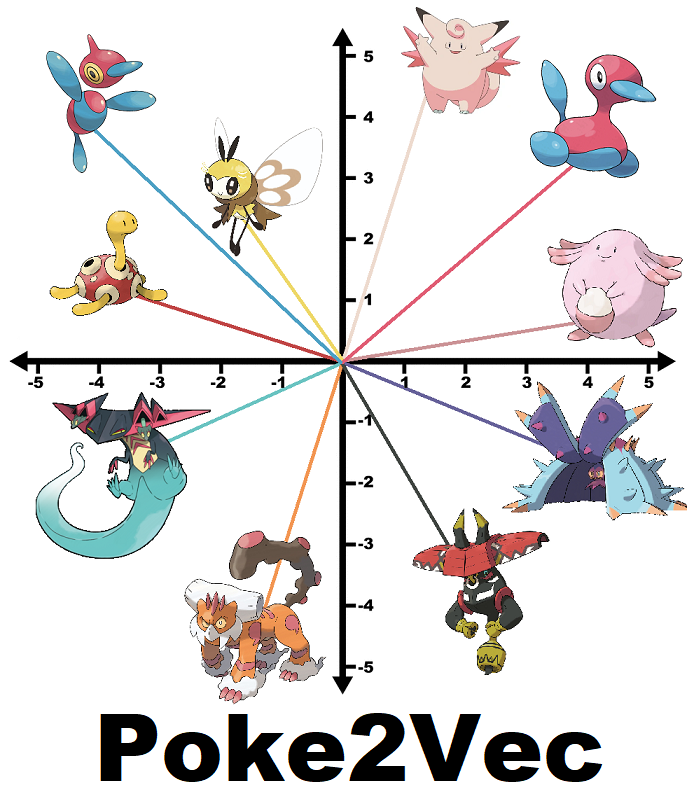
\includegraphics{header.png}

\hypertarget{introduction-background}{%
\subsection{Introduction / Background}\label{introduction-background}}

For people unfamiliar with the `2vec' kinds of models, the idea is to go
from a one-hot encoded representation (each pokemon corresponds to an 1
in an otherwise entirely 0 vector) to a lower-dimensional one that has
some useful information `baked' into it.

Word2Vec uses the idea that a word is defined by the context it appears
in.
\href{https://israelg99.github.io/2017-03-23-Word2Vec-Explained/}{Here}
is a helpful link that explains Word2Vec in case you're interested.
Expanding a bit, this means that words appearing in the same contexts
convey similar meaning. Taken this way, it's not super unreasonable to
expand this idea to Pokemon, since Pokemon that fill similar `roles'
within a team would probably find themselves having similar teammates. I
will be using data from battles hosted on Pokemon Showdown (PS), an
online Pokemon battling simulator.

\hypertarget{model-and-data-generation}{%
\subsection{Model and Data Generation}\label{model-and-data-generation}}

This part is a bit technical so for people who don't care about the gory
details about ``how'' please skip to the
\protect\hyperlink{Results}{Results} section.

\hypertarget{model}{%
\paragraph{Model}\label{model}}

The model I've described above (a word/pokemon being `defined' by the
words appearing in its context without consideration of position) is
referred to as a Continuous Bag-of-Words approach. There are a lot of
different ways to fit such a model, the way I've done it is using a
two-hidden layer neural network to get two matrices of `encodings' and
`decodings', and then average the resulting vectors element-wise to get
the final embedding.

\hypertarget{data-generation---theory}{%
\subsection{Data Generation - Theory}\label{data-generation---theory}}

n an ideal world, I would have access to the actual teams that were used
on PS in a given month. In the real world, I do not have access to this
data, so I have to estimate it.

The monthly usage statistics files give access to the marginal (eg:
\(P(Clefable \text{ on team})\)) and pairwise conditional (eg:
\(P(Charizard \text{ on team | } Clefable \text{ on team})\))
probabilities for all pokemon in the metagame. The problem is, the
actual probability of a team cannot be inferred from this, so
(incorrect) simplifying assumptions had to be made. This next section
goes into more technical detail about why this happens/what assumptions
end up being made, so unless you really care about statistics skip ahead
and take for granted that you can get the probability of a certain team
composition.

A joint probability, \(P(A & B & C)\), can (repeatedly) be broken down
into a marginal and conditional probability as shown below \[
P(A & B & C) = P(A & B | C) * P(C)
\] Using pokemon in place of random, you get \[
P(Spinda & Clefable & Bisharp) = P(Spinda & Clefable | Bisharp) * P(Bisharp)
\]

From the usage statistics, we have the marginal probability for Bisharp.
What we are missing is the conditional joint
\(P(Spinda & Clefable | Bisharp)\), all we have is
\(P(Spinda | Bisharp)\) and \(P(Clefable | Bisharp)\). A potential
work-around is to simply use the product of the two conditionals as an
approximation of the joint conditional, which statistically means that I
am making an assumption about the conditional independence of two
events. Specifically, this assumption means that, given Bisharp is
already on a team, the events of Clefable being on the team and Spinda
being on the team are independent. Mathematically, this corresponds to
the following equations \[
P(Spinda & Clefable & Bisharp) = P(Spinda & Clefable | Bisharp) * P(Bisharp)
P(Spinda & Clefable & Bisharp) ≈ P(Spinda | Bisharp) * P(Clefable | Bisharp) * P(Bisharp)
\]

Where the independence assumption is used to decompose
\(P(Spinda & Clefable | Bisharp)\) as \[
P(Spinda & Clefable | Bisharp) = P(Spinda | Clefable, Bisharp) * P(Clefable | Bisharp)
P(Spinda & Clefable | Bisharp) = P(Spinda | Bisharp) * P(Clefable | Bisharp)
\]

\hypertarget{Results}{%
\subsection{Results}\label{Results}}

doot doot

\end{document}
